\documentclass[addpoints,spanish, 12pt,a4paper]{exam}
%\documentclass[answers, spanish, 12pt,a4paper]{exam}
\printanswers
\pointpoints{punto}{puntos}
\hpword{Puntos:}
\vpword{Puntos:}
\htword{Total}
\vtword{Total}
\hsword{Resultado:}
\hqword{Ejercicio:}
\vqword{Ejercicio:}

\usepackage[utf8]{inputenc}
\usepackage[spanish]{babel}
\usepackage{eurosym}
%\usepackage[spanish,es-lcroman, es-tabla, es-noshorthands]{babel}


\usepackage[margin=1in]{geometry}
\usepackage{amsmath,amssymb}
\usepackage{multicol}
\usepackage{yhmath}

\pointsinrightmargin % Para poner las puntuaciones a la derecha. Se puede cambiar. Si se comenta, sale a la izquierda.
\extrawidth{-2.4cm} %Un poquito más de margen por si ponemos textos largos.
\marginpointname{ \emph{\points}}

\usepackage{graphicx}

\graphicspath{{../../img/}} 

\newcommand{\class}{2º Bachillerato CIT}
\newcommand{\examdate}{\today}
\newcommand{\examnum}{Final 1ªEv.}
\newcommand{\tipo}{A}


\newcommand{\timelimit}{105 minutos}

\renewcommand{\solutiontitle}{\noindent\textbf{Solución:}\enspace}


\pagestyle{head}
\firstpageheader{
\includegraphics[width=0.2\columnwidth]{header_left}}{\textbf{Departamento de Matemáticas\linebreak \class}\linebreak \examnum}{
\includegraphics[width=0.1\columnwidth]{header_right}}
\runningheader{\class}{\examnum}{Página \thepage\ of \numpages}
\runningheadrule


\usepackage{pgf,tikz,pgfplots}
\pgfplotsset{compat=1.15}
\usepackage{mathrsfs}
\usetikzlibrary{arrows}


\begin{document}

\noindent
\begin{tabular*}{\textwidth}{l @{\extracolsep{\fill}} r @{\extracolsep{6pt}} }
\textbf{Nombre:} \makebox[3.5in]{\hrulefill} & \textbf{Fecha:}\makebox[1in]{\hrulefill} \\
 & \\
\textbf{Tiempo: \timelimit} & Tipo: \tipo 
\end{tabular*}
\rule[2ex]{\textwidth}{2pt}
Esta prueba tiene \numquestions\ ejercicios. La puntuación máxima es de \numpoints. 
La nota final de la prueba será la parte proporcional de la puntuación obtenida sobre la puntuación máxima. 

\begin{center}


\addpoints
 %\gradetable[h][questions]
	\pointtable[h][questions]
\end{center}

\noindent
\rule[2ex]{\textwidth}{2pt}

\begin{questions}


\question[6] Calcula el siguiente límite: $$\lim_{x \to 1} \left(\frac{x^{3} - 2 x + 2}{3 x^{2} - 2}\right)^{\frac{x^{2} - 3 x}{x^{2} + x - 2}}$$
\begin{solution}
$\lim_{x \to 1} \left(\frac{x^{3} - 2 x + 2}{3 x^{2} - 2}\right)^{\frac{x^{2} - 3 x}{x^{2} + x - 2}}=1^\infty$. Indeterminación \\ $g(x)\cdot\left[f(x)-1\right]=\frac{x \left(x - 3\right)}{\left(x - 1\right) \left(x + 2\right)}\cdot\frac{\left(x - 1\right) \left(x^{2} - 2 x - 4\right)}{3 x^{2} - 2}=\frac{x \left(x - 3\right) \left(x^{2} - 2 x - 4\right)}{\left(x + 2\right) \left(3 x^{2} - 2\right)}$. \\ $\lim_{x \to 1}\frac{x \left(x - 3\right) \left(x^{2} - 2 x - 4\right)}{\left(x + 2\right) \left(3 x^{2} - 2\right)}=\frac{10}{3}$. Por tanto: \\ $\lim_{x \to 1} \left(\frac{x^{3} - 2 x + 2}{3 x^{2} - 2}\right)^{\frac{x^{2} - 3 x}{x^{2} + x - 2}}=e^{\frac{10}{3}}$

\end{solution}
\addpoints

\question[6] Determine qué valor debe tomar k para que: $$\lim_{x \to +\infty}2x-\sqrt{4x^2+kx-5}=1$$
\begin{solution}
$\lim_{x \to +\infty}2x-\sqrt{4x^2+kx-5}=\lim_{x \to +\infty}\dfrac{(2x-\sqrt{4x^2+kx-5})\cdot(2x+\sqrt{4x^2+kx-5})}{(2x+\sqrt{4x^2+kx-5})}=\lim_{x \to +\infty}\dfrac{4x^2-4x^2-kx+5}{(2x+\sqrt{4x^2+kx-5})}=\lim_{x \to +\infty}\dfrac{-kx+5}{(2x+\sqrt{4x^2+kx-5})}=\lim_{x \to +\infty}\dfrac{-k+\frac{5}{x}}{(2+\sqrt{4+\frac{k}{x})-\frac{5}{x^2}}}=\dfrac{-k}{2+2} \to k = -4$
\end{solution}

\question[4] Hallar los puntos de la gráfica $y=2 x^{3} + 3 x^{2} - 30 x - 6$ en los que la recta tangente es paralela a la recta $y=6 x - 5$
\begin{solution}$f'(x)=6 x^{2} + 6 x - 30\land m=6$. Luego: \\ $6 x^{2} + 6 x - 30 = 6 \to x =\left[ -3, \  2\right] $. \ Los puntos de la gráfica son: \\   $\left(-3,57 \right)$ . \\  $\left(2,-38 \right)$ . \\ 
\end{solution}
\addpoints

\question Halla la derivada:

\begin{parts}
\part[6] $y=\ln{\left(\sqrt{\dfrac{\cos{\left(x \right)} + 1}{1 - \cos{\left(x \right)}}} \right)}$
\begin{solution}
$f'(x)=\left(- \frac{\log{\left(1 - \cos{\left(x \right)} \right)}}{2} + \frac{\log{\left(\cos{\left(x \right)} + 1 \right)}}{2}\right)^{'}=- \frac{\sin{\left(x \right)}}{2 \left(\cos{\left(x \right)} + 1\right)} - \frac{\sin{\left(x \right)}}{2 \left(1 - \cos{\left(x \right)}\right)}=\frac{\sin{\left(x \right)}}{\left(\cos{\left(x \right)} - 1\right) \left(\cos{\left(x \right)} + 1\right)}=- \frac{1}{\sin{\left(x \right)}}$
\end{solution}

% \part[7] $y=\dfrac{x \sqrt{x^{2} - 1}}{2} - \tan{\left(x + \sqrt{x^{2} - 1} \right)}$
% \begin{solution}


% $f'(x)=\left(\frac{x \sqrt{x^{2} - 1}}{2}\right)^{'}+\left(- \tan{\left(x + \sqrt{x^{2} - 1} \right)}\right)^{'}=\frac{2x^{2} - 1}{2\sqrt{x^{2} - 1}}- \frac{\left(x + \sqrt{x^{2} - 1}\right) \left(\sec^{2}{\left(x + \sqrt{x^{2} - 1} \right)} \right)}{\sqrt{x^{2} - 1}}=\frac{2 x^{2} - 2 \left(x + \sqrt{x^{2} - 1}\right) \sec^{2}{\left(x + \sqrt{x^{2} - 1} \right)}-1}{2 \sqrt{x^{2} - 1}}
% $

% \end{solution}

\end{parts}
\addpoints


\question[4] Determina a y b para que sea derivable en $\mathbb{R}$ la función: $$f(x)=\left\{\begin{matrix}
\ln{\left(\sen{\left(x \right)} + e \right)} & si & x<0 \\
a x + b + x^{3} & si & x\geqslant 0 \\
\end{matrix}\right.$$ 


\begin{solution}
Continuidad en 0:\\ $\lim_{x \to 0^-} \log{\left(\sin{\left(x \right)} + e \right)} = \lim_{x \to 0^+}\left(a x + b + x^{3}\right) \to 1 = b $ \\ Derivabilidad en 0: \\ $\lim_{x \to 0^-}\left(\frac{\cos{\left(x \right)}}{\sin{\left(x \right)} + e}\right) = \lim_{x \to 0^+}\left(a + 3 x^{2}\right) \to e^{-1} = a $ \\ Por tanto: $\left\{ a : e^{-1}, \  b : 1\right\} $ \\ 
\end{solution}

\addpoints

% \question[6] Aprovechando como hipotenusa una pared de $10 \sqrt{2}$ m. se desea acotar una superficie triangular de área máxima.¿Qué medidas deberán tener los otros dos lados (catetos)?
% \begin{solution}
% Función a optimizar: $\frac{x \sqrt{200 - x^{2}}}{2}$ \\ $f'(x)=\frac{100 - x^{2}}{\sqrt{200 - x^{2}}}\land f''(x)=\frac{x \left(x^{2} - 300\right)}{\left(200 - x^{2}\right)^{\frac{3}{2}}}$ \\ Extremos relativos: \\ $-10\land f''(-10)=2$ \\ $10\land f''(10)=-2$ \\
% \end{solution}

\addpoints

\question Dada la función: $$f(x)=\dfrac{x^2}{x-8}$$
\begin{parts}
\part[4] Determinar los intervalos de crecimiento y decrecimiento
\begin{solution}
$(-\infty, 0) \cup (16,\infty)$ creciente. \\
$(0,8) \cup (8,16)$ decreciente.
\end{solution}
\part[2] Hallar los máximos y mínimos relativos de la función
\begin{solution}
$f(x)$ es continua en $\mathbb{R}-\left\{8\right\}$. \\
$f'(x)=0 \to \frac{x \left(x - 16\right)}{\left(x - 8\right)^{2}}=0  \to x=0 \land x=16$. \\
$(0, f(0))=(0,0) \land (16,f(16))=(16,32)$ \\
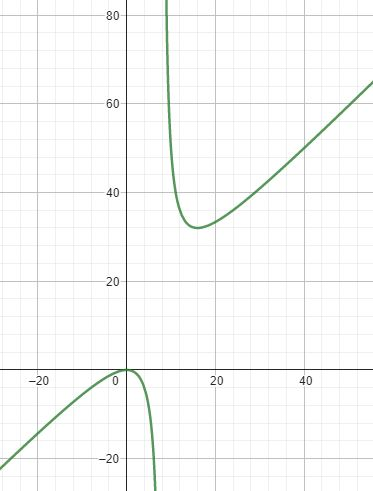
\includegraphics[scale=0.30]{2bac/2bac_cie/funcion2.jpg}
\end{solution}
\part[4] Determina las asíntotas de la gráfica de $f(x)$
\begin{solution}
$x=8$ Asíntota vertical \\
$\lim_{x \to \infty}\frac{f(x)}{x}=1$ \\
$\lim_{x \to \infty}f(x)-1\cdot x=8$ \\
$y=x+8$ Asíntota oblicua
\end{solution}

\part[2] Calcula, razonadamente, el máximo y el mínimo absoluto 
\begin{solution}
$$\lim_{x \to 8^-}\left(\frac{x^{2}}{x - 8}\right)=-\infty \to (8,-\infty)$$
$$\lim_{x \to 8^-}\left(\frac{x^{2}}{x - 8}\right)=+\infty \to (8,\infty)$$
\end{solution}
\end{parts}


% \question Dada la función: $f(x)=x + e^{- x}$ 
% \begin{parts}
% \part[5] Determina los intervalos de crecimiento y decrecimiento de f, así como los extremos relativos (máximos o mínimos)
% \begin{solution}
% $dom(f(x))=\mathbb{R}$ \\
% $f'(x)=1 - e^{- x} \to f'(x)=0 \to 1 - e^{- x} = 0 \to x=0 $  \\
% Intervalos de crecimiento: $\left[ \left[ \left(-\infty, 0\right), \  \text{False}\right], \  \left[ \left(0, \infty\right), \  \text{True}\right]\right]$ \\
% \end{solution}
% % \part[5] Determina los intervalos de concavidad y convexidad de f
% % \begin{solution}$f''(x)=e^{- x} \to f''(x)>0$ \\ Intervalos de convexidad:$\left[ \mathbb{R}, \  \text{True}\right]$ \\ 
% % \end{solution}
% \part[5] Determina las asíntotas de la gráfica de f
% \begin{solution}
% $dom(f(x))=\mathbb{R} \to \nexists A.V.$ \\
% $lim_{x \to +\infty} f(x)= \infty + 0 = \infty \land lim_{x \to -\infty} f(x)= -\infty \to \nexists A.H.$ \\
% Asíntota oblícua: \\ 

% pendiente: $lim_{x \to \infty}\frac{f(x)}{x}=lim_{x \to \infty}1+ \frac{e^{-x}}{x} = 1$ \\
% ordenada: $lim_{x \to \infty}f-m\cdot x=lim_{x \to \infty}e^{-x}=0 \to A.O: y=x$

% \end{solution}
% \end{parts}

\addpoints

\question[4] Demuestra, razonadamente, que la función $g(x)=x^3+2x$ vale $4$ para algún valor de $x \in \left[1,2\right]$.
\begin{solution} Sea $f(x)=x^3+2x-4 \to f(1)=1+2-4=-1 <0 \land f(2)=8+4-4=8>0 \land $ f es continua en $\mathbb{R}$. Aplicando Bolzano  $\to \exists x \in \left[1,2 \right], f(x)=0 \to g(x)=4$\end{solution}



\question[4] OJO, está mal (no entra en EVAU). Determine el límite siguiente: 
$$\lim_{x \to \frac{\pi}{2}} \left(\dfrac{1}{1-\sen{x}}\right)^\frac{\cos{x}}{\sen{x}}$$

\begin{solution}
$\lim_{x \to \frac{\pi}{2}} \left(\dfrac{1}{1-\sen{x}}\right)^\frac{\cos{x}}{\sen{x}}=
e^{\lim_{x \to \frac{\pi}{2}} \left(\dfrac{1}{1-\sen{x}}-1\right)\cdot\frac{\cos{x}}{\sen{x}}}=
e^{\lim_{x \to \frac{\pi}{2}} \left(\dfrac{\sen{x}}{1-\sen{x}}\right)\cdot\frac{\cos{x}}{\sen{x}}}=
e^{\lim_{x \to \frac{\pi}{2}} \left(\dfrac{\cos{x}}{1-\sen{x}}\right)}=e^1=e
$

\end{solution}

% % \question Se define la función f del modo siguiente:

% % $$f(x)=\left\{\begin{matrix}
% % \ln{x} -1   & si & x>1 \\
% % 2 x^2 + ax + b & si & x\leqslant 1 \\
% % \end{matrix}\right.$$
% % \begin{parts}
% % \part[] Encontrar los valores de a y b para que la función sea continua y su gráfica pase por el origen de
% % coordenadas.
% % \part[] Estudiar su derivabilidad
% % \part[2] Hallar los puntos de su gráfica en los que
% % la tangente es paralela al eje OX
% % \end{parts}
% % \begin{solution}
% % a = -3 , b = 0. Derivable en R. x=3/4
% % \end{solution}

% %\question 
% %
% %\begin{parts}
% %\part[2] 
% %\begin{solution}
% %\end{solution}
% %
% %
% %\end{parts}
% %\addpoints

% \question[2] Halla el valor de $a$ para el cual la función $f(x)=\dfrac{x^2+x+a}{x^2+3x-4}$ tenga una discontinuidad evitable en $x=1$.


% \question Dada la función $y=x+\dfrac{4}{(x-1)^2}$, calcula:
% \begin{parts}
% \part[4] Dominio de la función y asíntotas
% \part[4] Intervalos de crecimiento y decrecimiento
% \end{parts}

% \question[4] Halla la derivada de  $y=\dfrac{x \sqrt{x^{2} - 1}}{2} - \tg{\left(x + \sqrt{x^{2} - 1} \right)}$
% \begin{solution}


% $f'(x)=\left(\frac{x \sqrt{x^{2} - 1}}{2}\right)^{'}+\left(- \tan{\left(x + \sqrt{x^{2} - 1} \right)}\right)^{'}=\frac{2x^{2} - 1}{2\sqrt{x^{2} - 1}}- \frac{\left(x + \sqrt{x^{2} - 1}\right) \left(\sec^{2}{\left(x + \sqrt{x^{2} - 1} \right)} \right)}{\sqrt{x^{2} - 1}}=\frac{2 x^{2} - 2 \left(x + \sqrt{x^{2} - 1}\right) \sec^{2}{\left(x + \sqrt{x^{2} - 1} \right)}-1}{2 \sqrt{x^{2} - 1}}
% $

% \end{solution}

% \question Dada la función $f(x)=\dfrac{2x^2-3x}{e^x}$:
% \begin{parts}
% \part[4] Estudia los intervalos de crecimiento y decrecimiento
% \part[2] Determina, si existen, sus máximos y mínimos relativos
% \end{parts}

% \question[2] Demuestra que la función $f(x)=x^3-8x+2$ corta al eje de abscisas en el intervalo $\left(0,2\right)$


% \question Dada $f(x)=\dfrac{|x-1|}{x}$:
% \begin{parts}
% \part[2] Estudiar la derivabilidad de $f$
% \part[2] Tiene la función máximos o mínimos relativos. Razona tu respuesta
% \end{parts}

% \question[4] Hallar $a>0$ y $b>0$ sabiendo que en el punto $P(1,2)$ la recta tangente a la gráfica de la función $f(x)=\dfrac{bx^2}{1+ax^4}$  es horizontal.
% \begin{solution}
% $f'(x)=- \frac{2 b x \left(a x^{4} - 1\right)}{\left(a x^{4} + 1\right)^{2}}\to$\\
% $f'(1)=0 \to \left(a \cdot 1^{4} - 1\right)=0 \to a =1 $\\
% $f(1)=2 \to \frac{b\cdot1^{2}}{1^{4} + 1}=2 \to b=4$\\
% $a=1$, $b=4$.
% \end{solution}



\end{questions}

\end{document}
\grid
